\documentclass[../main.tex]{subfiles}



\begin{document}

\chapter{}
\label{cha:cha_4}


\section{}
The true value can be computed as
\bigbreak
$f^{\prime}(1.22)=\dfrac{6(0.577)}{\left(1-3 \times 0.577^{2}\right)^{2}}=2,352,911$
\bigbreak
Using 3-digits with chopping
\bigbreak
$
\begin{aligned}
&6 x=6(0.577)=3.462 \underset{\text { chopping }}{\longrightarrow} 3.46 \\
&x=0.577 \\
&x^{2}=0.332929 \stackrel{\text { chopping }}{\longrightarrow} 0.332 \\
&3 x^{2}=0.996 \\
&1-3 x^{2}=0.004 \\ \\
&f^{\prime}(0.577)=\dfrac{3.46}{(1-0.996)^{2}}=\dfrac{3.46}{0.004^{2}}=216,250
\end{aligned}
$
\bigbreak
This represents a percent relative error of
\bigbreak
$\varepsilon_{t}=\left|\dfrac{2,352,911-216,250}{2,352,911}\right|=90.8 \%$
\bigbreak
Using 4-digits with chopping
\bigbreak
$
\begin{aligned}
&6 x=6(0.577)=3.462 \stackrel{\text { chopping }}{\longrightarrow} 3.462 \\
&x=0.577 \\
&x^{2}=0.332929 \stackrel{\text { chopping }}{\longrightarrow} 0.3329 \\
&3 x^{2}=0.9987 \\
&1-3 x^{2}=0.0013 \\
&f^{\prime}(0.577)=\dfrac{3.462}{(1-0.9987)^{2}}=\dfrac{3.462}{0.0013^{2}}=2,048,521
\end{aligned}
$
\bigbreak
This represents a percent relative error of
\bigbreak
$\varepsilon_{t}=\left|\dfrac{2,352,911-2,048,521}{2,352,911}\right|=12.9 \%$
\bigbreak
Although using more significant digits improves the estimate, the error is still considerable. The problem stems primarily from the fact that we are subtracting two nearly equal numbers in the denominator. Such subtractive cancellation is worsened by the fact that the denominator is squared.
\bigbreak
\section{}
First, the correct result can be calculated as
\bigbreak
$y=1.37^{3}-7(1.37)^{2}+8(1.37)-0.35=0.043053$
\bigbreak
\begin{enumerate}[label=\bfseries(\alph*)]
\item Using 3-digits with chopping
\bigbreak
$\begin{array}{llllc}1.37^{3} & \rightarrow & 2.571353 & \rightarrow & 2.57 \\ -7(1.37)^{2} & \rightarrow & -7(1.87) & \rightarrow & -13.0 \\ 8(1.37) & \rightarrow & 10.96 & \rightarrow & 10.9 \\ & & & &\underline{ -0.35} \\ & & & & -0.12\end{array}$
\bigbreak
This represents an error of
\bigbreak
$\varepsilon_{t}=\left|\dfrac{0.043053-0.12}{0.043053}\right|=178.7 \%$
\bigbreak
\item Using 3-digits with chopping
\bigbreak
$
\begin{aligned}
&y=((1.37-7) 1.37+8) 1.37 - 0.35\\
&y=(-5.63 \times 1.37+8) 1.37  - 0.35\\
&y=(-7.71+8) 1.37-0.35 \\
&y=0.29 \times 1.37-0.35 \\
&y=0.397-0.35 \\
&y=0.047
\end{aligned}
$
\bigbreak
This represents an error of
\bigbreak
$\varepsilon_{t}=\left|\dfrac{0.043053-0.47}{0.043053}\right|=9.2 \%$
\bigbreak
Hence, the second form is superior because it tends to minimize round-off error.
\bigbreak
\end{enumerate}
\section{}
\begin{enumerate}[label=\bfseries(\alph*)]
\item For this case, $x_{i}=0$ and $h=x$. Thus, the Taylor series is
\bigbreak
$f(x)=f(0)+f^{\prime}(0) x+\dfrac{f^{\prime \prime}(0)}{2 !} x^{2}+\dfrac{f^{(3)}(0)}{3 !} x^{3}+\cdots$
\bigbreak
For the exponential function,
\bigbreak
$f(0)=f^{\prime}(0)=f^{\prime \prime}(0)=f^{(3)}(0)=1$
\bigbreak
Substituting these values yields,
\bigbreak
 $f(x)=1+x+\dfrac{1}{2 !} x^{2}+\dfrac{1}{3 !} x^{3}+\cdots$
 \bigbreak
which is the Maclaurin series expansion.
\bigbreak
\item  The true value is $e^{-1}=0.367879$ and the step size is $h=x_{i+1}-x_{i}=1-0.25=0.75$. The complete Taylor series to the third-order term is
\bigbreak
$f\left(x_{i+1}\right)=e^{-x_{i}}-e^{-x_{i}} h+e^{-x_{i}} \dfrac{h^{2}}{2}-e^{-x_{i}} \dfrac{h^{3}}{3 !}$
\bigbreak
Zero-order approximation:
\bigbreak
$f(1)=e^{-0.25}=0.778801$
\bigbreak
$\varepsilon_{t}=\left|\dfrac{0.367879-0.778801}{0.367879}\right| 100 \%=111.7 \%$
\bigbreak
First-order approximation:
\bigbreak
$
\begin{aligned}
&f(1)=0.778801-0.778801(0.75)=0.19 \\ \\
&\varepsilon_{t}=\left|\dfrac{0.367879-0.1947}{0.367879}\right| 100 \%=47.1 \%
\end{aligned}
$
\bigbreak
Second-order approximation:
\bigbreak
$
\begin{aligned}
&f(1)=0.778801-0.778801(0.75)+0.778801 \dfrac{0.75^{2}}{2}=0.41 \\ \\
&\varepsilon_{t}=\left|\dfrac{0.367879-0.413738}{0.367879}\right| 100 \%=12.5 \%
\end{aligned}
$
\bigbreak
Third-order approximation:
\bigbreak
$
\begin{aligned}
&f(1)=0.778801-0.778801(0.75)+0.778801 \dfrac{0.75^{2}}{2}-0.778801 \dfrac{0.75^{3}}{6}=0.3589 \\ \\
&\varepsilon_{t}=\left|\dfrac{0.367879-0.358978}{0.367879}\right| 100 \%=2.42 \%
\end{aligned}
$
\bigbreak
\section{}
Use $\varepsilon_{\mathrm{s}}=0.5 \times 10^{2-2}=0.5 \%$. The true value $=\cos (\pi / 4)=0.707107 \ldots$
\bigbreak
zero-order: 
\bigbreak
$\cos \left(\dfrac{\pi}{4}\right) \cong 1$
\bigbreak
$\varepsilon_{t}=\left|\dfrac{0.707107-1}{0.707107}\right| 100 \%=41.42 \%$
\bigbreak
first-order:
\bigbreak
$\cos \left(\dfrac{\pi}{4}\right) \cong 1-\dfrac{(\pi / 4)^{2}}{2}=0.691575$
\bigbreak
$\varepsilon_{t}=\left|\dfrac{0.707107-0.691575}{0.707107}\right| 100 \%=2.19 \%$
\bigbreak
$\varepsilon_{a}=\left|\dfrac{0.691575-1}{0.691575}\right| 100 \%=44.6 \%$
\bigbreak

second-order:
\bigbreak
$\cos \left(\dfrac{\pi}{4}\right) \cong 0.691575+\dfrac{(\pi / 4)^{4}}{24}=0.707429$
\bigbreak
$\varepsilon_{t}=\left|\dfrac{0.707107-0.707429}{0.707107}\right| 100 \%=0.456 \%$
\bigbreak
$\varepsilon_{a}=\left|\dfrac{0.707429-0.691575}{0.707429}\right| 100 \%=2.24 \%$
\bigbreak

third-order:
\bigbreak
$\cos \left(\dfrac{\pi}{4}\right) \cong 0.707429-\dfrac{(\pi / 4)^{6}}{720}=0.707103$
\bigbreak
$\varepsilon_{t}=\left|\dfrac{0.707107-0.707103}{0.707107}\right| 100 \%=0.0005 \%$
\bigbreak
$\varepsilon_{a}=\left|\dfrac{0.707103-0.707429}{0.707103}\right| 100 \%=0.046 \%$
\bigbreak
Because $\varepsilon_{a}<0.5 \%$, we can terminate the computation.
\bigbreak


\section{}
Use $\varepsilon_{\mathrm{s}}=0.5 \times 10^{2-2}=0.5 \%$. The true value $=\sin (\pi / 4)=0.707107 \ldots$
\bigbreak
zero-order: 
\bigbreak
$\sin \left(\dfrac{\pi}{4}\right) \cong 0.785398$
\bigbreak

$\varepsilon_{t}=\left|\dfrac{0.707107-0.785398}{0.707107}\right| 100 \%=11.1 \%$
\bigbreak
first-order:
\bigbreak
$\sin \left(\dfrac{\pi}{4}\right) \cong 0.785398-\dfrac{(\pi / 4)^{3}}{6}=0.704653$
\bigbreak
$\varepsilon_{t}=\left|\dfrac{0.707107-0.704653}{0.707107}\right| 100 \%=0.347 \%$
\bigbreak
$\varepsilon_{a}=\left|\dfrac{0.704653-0.785398}{0.704653}\right| 100 \%=11.46 \%$
\bigbreak
second-order:
\bigbreak
$\sin \left(\dfrac{\pi}{4}\right) \cong 0.704653+\dfrac{(\pi / 4)^{5}}{120}=0.707143$
\bigbreak
$\varepsilon_{t}=\left|\dfrac{0.707107-0.707143}{0.707107}\right| 100 \%=0.0051 \%$
\bigbreak
$\varepsilon_{a}=\left|\dfrac{0.707143-0.704653}{0.707143}\right| 100 \%=0.352 \%$
\bigbreak
Because $\varepsilon_{a}<0.5 \%$, we can terminate the computation.
\bigbreak


\section{}

The true value is $f(2)=102$.
\bigbreak
zero order:
\bigbreak
$f(2)=f(1)=-62 \quad\quad\quad\quad\quad\varepsilon_{t}=\left|\dfrac{102-(-62)}  {102}\right| 100 \%=160.8 \%$
\bigbreak
first order:
\bigbreak
$
\begin{aligned}
& f^{\prime}(1)=75(1)^{2}-12(1)+7=70 \\ \\
& f(2)=-62+70(1)=8 \quad\quad\quad\quad\quad \varepsilon_{t}=\left|\dfrac{102-8}{102}\right| 100 \%=92.1 \% 
\end{aligned}
$
\bigbreak
second order:
\bigbreak

$
\begin{aligned}
&f^{\prime \prime}(1)=150(1)-12=138 \\ \\
&f(2)=8+\dfrac{138}{2}(1)^{2}=77 \quad\quad\quad\quad\varepsilon_{t}=\left|\dfrac{102-77}{102}\right| 100 \%=24.5 \%
\end{aligned}
$
\bigbreak
third order:
\bigbreak
$
\begin{aligned}
&f^{(3)}(1)=150 \\ \\
&f(2)=77+\dfrac{150}{6}(1)^{3}=102 \quad\quad\quad\quad \varepsilon_{t}=\left|\dfrac{102-102}{102}\right| 100 \%=0.0 \%
\end{aligned}
$
\bigbreak
Because we are working with a third-order polynomial, the error is zero. This is due to the fact that cubics have zero fourth and higher derivatives.
\bigbreak

\section{}
The true value is $\ln (3)=1.098612$
\bigbreak
zero order:
\bigbreak
$f(3)=f(1)=0 \quad\quad\quad\quad\quad \varepsilon_{t}=\left|\dfrac{1.098612-0}{1.098612}\right| 100 \%=100 \%$
\bigbreak
first order:
\bigbreak$
\begin{aligned}
&f^{\prime}(x)=\dfrac{1}{x}  \quad\quad\quad f^{\prime}(1)=1 \\\\
&f(3)=0+1(2)=2 \quad\quad\quad\quad\quad \varepsilon_{t}=\left|\dfrac{1.098612-2}{1.098612}\right| 100 \%=82.05 \%
\end{aligned}$
\bigbreak
second order:
\bigbreak$
\begin{aligned}
&f^{\prime \prime}(x)=-\dfrac{1}{x^{2}} \quad\quad \quad f^{\prime \prime}(1)=-1 \\\\
&f(3)=2-1 \dfrac{2^{2}}{2}=0 \quad\quad\quad\quad\quad \varepsilon_{t}=\left|\dfrac{1.098612-0}{1.098612}\right| 100 \%=100 \%
\end{aligned}$
\bigbreak
third order:
\bigbreak$
\begin{aligned}
&f^{(3)}(x)=\dfrac{2}{x^{3}} \quad \quad\quad f^{\prime \prime}(1)=2 \\\\
&f(3)=0+2 \dfrac{2^{3}}{6}=2.66667 \quad\quad\quad\quad\quad \varepsilon_{t}=\left|\dfrac{1.098612-2.66667}{1.098612}\right| 100 \%=142.7 \%
\end{aligned}$
\bigbreak
fourth order:
\bigbreak$
\begin{aligned}
&f^{(4)}(x)=-\dfrac{6}{x^{4}}\quad \quad \quad f^{(4)}(1)=-6 \\\\
&f(3)=2.66666-6 \dfrac{2^{4}}{24}=-1.33333 \quad\quad\quad\quad\quad \varepsilon_{t}=\left|\dfrac{1.098612-(-1.33333)}{1.098612}\right| 100 \%=221.4 \%
\end{aligned}$
\bigbreak
The series is diverging. A smaller step size is required to obtain convergence.
\bigbreak


\section{}

The first derivative of the function at $x=2$ can be evaluated as
\bigbreak
$f^{\prime}(2)=75(2)^{2}-12(2)+7=283$
\bigbreak
The points needed to form the finite divided differences can be computed as
\bigbreak$
\begin{array}{ll}
x_{i-1}=1.75 \quad\quad\quad& f\left(x_{i-1}\right)=39.85938 \\
x_{i}=2.0\quad\quad\quad & f\left(x_{i}\right)=102 \\
x_{i+1}=2.25 \quad\quad\quad& f\left(x_{i+1}\right)=182.1406
\end{array}$
\bigbreak
forward:
\bigbreak
$f^{\prime}(2)=\dfrac{182.1406-102}{0.25}=320.5625 \quad\quad\quad\left|E_{t}\right|=|283-320.5625|=37.5625$
\bigbreak
backward:
\bigbreak
$f^{\prime}(2)=\dfrac{102-39.85938}{0.25}=248.5625 \quad\quad\quad\left|E_{t}\right|=|283-248.5625|=34.4375$
\bigbreak
centered:
\bigbreak
$f^{\prime}(2)=\dfrac{182.1406-39.85938}{0.5}=284.5625\quad\quad \quad E_{t}=283-284.5625=-1.5625$
\bigbreak
Both the forward and backward differences should have errors approximately equal to
\bigbreak
$\left|E_{t}\right| \approx \dfrac{f^{\prime \prime}\left(x_{i}\right)}{2} h$
\bigbreak
The second derivative can be evaluated as
\bigbreak
$f^{\prime \prime}(2)=150(2)-12=288$
\bigbreak
Therefore,
\bigbreak
$\left|E_{t}\right| \approx \dfrac{288}{2} 0.25=36$
\bigbreak
which is similar in magnitude to the computed errors.
\bigbreak
For the central difference,
\bigbreak
$E_{t} \approx-\dfrac{f^{(3)}\left(x_{i}\right)}{6} h^{2}$
\bigbreak
The third derivative of the function is 150 and
\bigbreak
$E_{t} \approx-\dfrac{150}{6}(0.25)^{2}=-1.5625$
\bigbreak
which is exact. This occurs because the underlying function is a cubic equation that has zero fourth and higher derivatives.
\bigbreak


\section{}
The second derivative of the function at $x=2$ can be evaluated as
\bigbreak
$f^{\prime}(2)=150(2)-12=288$
\bigbreak
For $h=0.2,$
\bigbreak
$f^{\prime \prime}(2)=\dfrac{164.56-2(102)+50.96}{(0.2)^{2}}=288$
\bigbreak
For $h=0.1,$
\bigbreak
$f^{\prime \prime}(2)=\dfrac{131.765-2(102)+75.115}{(0.1)^{2}}=288$
\bigbreak
Both are exact because the errors are a function of fourth and higher derivatives which are zero for a $3^{\text {rd }}$-order polynomial.
\bigbreak


\section{}

Use $\varepsilon_{\mathrm{s}}=0.5 \times 10^{2-2}=0.5 \%$. The true value $=1 /(1-0.1)=1.11111 \ldots$
\bigbreak
zero-order:
\bigbreak
$\dfrac{1}{1-0.1} \cong 1$
\bigbreak
$\varepsilon_{t}=\left|\dfrac{1.11111-1}{1.11111}\right| 100 \%=10 \%$
\bigbreak
first-order:
\bigbreak
$\dfrac{1}{1-0.1} \cong 1+0.1=1.1$
\bigbreak$
\begin{aligned}
&\varepsilon_{t}=\left|\dfrac{1.11111-1.1}{1.11111}\right| 100 \%=1 \% \\\\
&\varepsilon_{a}=\left|\dfrac{1.1-1}{1.1}\right| 100 \%=9.0909 \%
\end{aligned}$
\bigbreak
second-order:
\bigbreak$
\begin{aligned}
&\dfrac{1}{1-0.1} \cong 1+0.1+0.01=1.11 \\\\
&\varepsilon_{t}=\left|\dfrac{1.11111-1.11}{1.11111}\right| 100 \%=0.1 \% \\\\
&\varepsilon_{a}=\left|\dfrac{1.11-1.1}{1.11}\right| 100 \%=0.9009 \%
\end{aligned}$
\bigbreak
third-order:
\bigbreak$
\begin{aligned}
&\dfrac{1}{1-0.1} \cong 1+0.1+0.01+0.001=1.111 \\\\
&\varepsilon_{t}=\left|\dfrac{1.11111-1.111}{1.11111}\right| 100 \%=0.01 \% \\\\
&\varepsilon_{a}=\left|\dfrac{1.111-1.11}{1.111}\right| 100 \%=0.090009 \%
\end{aligned}$
\bigbreak
The approximate error has fallen below $0.5 \%$ so the computation can be terminated.
\bigbreak


\section{}
Here are the function and its derivatives
\bigbreak$
\begin{aligned}
&f(x)=x-1-\dfrac{1}{2} \sin x \\
&f^{\prime}(x)=1-\dfrac{1}{2} \cos x \\
&f^{\prime \prime}(x)=\dfrac{1}{2} \sin x \\
&f^{(3)}(x)=\dfrac{1}{2} \cos x \\
&f^{(4)}(x)=-\dfrac{1}{2} \sin x
\end{aligned}$
\bigbreak
Using the Taylor Series expansion, we obtain the following $1^{\text {st }}, 2^{\text {nd }}, 3^{\text {rd }}$, and $4^{\text {th }}$ order Taylor Series functions shown below in the MATLAB program-$f1$, $f2$, and $f 4$. Note the $2^{\text {nd }}$ and $3^{\text {rd }}$ order Taylor Series functions are the same.
\bigbreak
From the plots below, we see that the answer is the \underline{$4^{\text {th }}$ Order Taylor Series expansion.}
\bigbreak
\begin{lstlisting}[numbers=none]
x=0:0.001:3.2;
f=x-1-0.5*sin(x);
subplot(2,2,1);
plot(x,f);grid;title('f(x)=x-1-0.5*sin(x)');hold on

f1=x-1.5;
e1=abs(f-f1);   %Calculates the absolute value of the
difference/error
subplot(2,2,2);
plot(x,e1);grid;title('1st Order Taylor Series Error');

f2=x-1.5+0.25.*((x-0.5*pi).^2);
e2=abs(f-f2);
subplot(2,2,3);
plot(x,e2);grid;title('2nd/3rd Order Taylor Series Error');

f4=x-1.5+0.25.*((x-0.5*pi).^2)-(1/48)*((x-0.5*pi).^4);
e4=abs(f4-f);
subplot(2,2,4);
plot(x,e4);grid;title('4th Order Taylor Series Error');hold off
\end{lstlisting}
\bigbreak
\begin{figure}[H]\quad\quad\quad\quad\quad\quad\quad\quad
		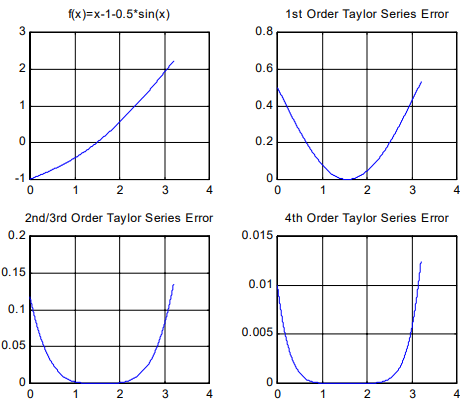
\includegraphics[width=0.7\linewidth]{fig_4_1}
		\label{fig:fig_4_1}
	\end{figure}
	\bigbreak
\section{}
\begin{tabular}{rrrrrrrrrr}
\multicolumn{1}{l}{$\underline{\mathbf{x}}$} & $\underline{\mathbf{f}(\mathbf{x})}$ & $\underline{\mathbf{f}(\mathbf{x}-\mathbf{1})}$ & $\underline{\mathbf{f}(\mathbf{x}+\mathbf{1})}$ & $\underline{\mathbf{f}^{\prime}(\mathbf{x}) \textbf {-Theory }}$ & $\underline{\mathbf{f}^{\prime}(\mathbf{x}) \textbf {-Back }}$ & $\underline{\mathbf{f}^{\prime}(\mathbf{x})-\mathbf{C e n t}}$ & $\underline{\mathbf{{f}^{\prime}(}\mathbf{{x})} \textbf {-Forw }}$ \\\\
$-2.000$ & $0.000$ & $-2.891$ & $2.141$ & $10.000$ & $11.563$ & $10.063$ & $8.563$ \\
$-1.750$ & $2.141$ & $0.000$ & $3.625$ & $7.188$ & $8.563$ & $7.250$ & $5.938$ \\
$-1.500$ & $3.625$ & $2.141$ & $4.547$ & $4.750$ & $5.938$ & $4.813$ & $3.688$ \\
$-1.250$ & $4.547$ & $3.625$ & $5.000$ & $2.688$ & $3.688$ & $2.750$ & $1.813$ \\
$-1.000$ & $5.000$ & $4.547$ & $5.078$ & $1.000$ & $1.813$ & $1.063$ & $0.313$ \\
$-0.750$ & $5.078$ & $5.000$ & $4.875$ & $-0.313$ & $0.313$ & $-0.250$ & $-0.813$ \\
$-0.500$ & $4.875$ & $5.078$ & $4.484$ & $-1.250$ & $-0.813$ & $-1.188$ & $-1.563$ \\
$-0.250$ & $4.484$ & $4.875$ & $4.000$ & $-1.813$ & $-1.563$ & $-1.750$ & $-1.938$ \\
$0.000$ & $4.000$ & $4.484$ & $3.516$ & $-2.000$ & $-1.938$ & $-1.938$ & $-1.938$ \\
$0.250$ & $3.516$ & $4.000$ & $3.125$ & $-1.813$ & $-1.938$ & $-1.750$ & $-1.563$ \\
$0.500$ & $3.125$ & $3.516$ & $2.922$ & $-1.250$ & $-1.563$ & $-1.188$ & $-0.813$ \\
$0.750$ & $2.922$ & $3.125$ & $3.000$ & $-0.313$ & $-0.813$ & $-0.250$ & $0.313$ \\
$1.000$ & $3.000$ & $2.922$ & $3.453$ & $1.000$ & $0.313$ & $1.063$ & $1.813$ \\
$1.250$ & $3.453$ & $3.000$ & $4.375$ & $2.688$ & $1.813$ & $2.750$ & $3.688$ \\
$1.500$ & $4.375$ & $3.453$ & $5.859$ & $4.750$ & $3.688$ & $4.813$ & $5.938$ \\
$1.750$ & $5.859$ & $4.375$ & $8.000$ & $7.188$ & $5.938$ & $7.250$ & $8.563$ \\
$2.000$ & $8.000$ & $5.859$ & $10.891$ & $10.000$ & $8.563$ & $10.063$ & $11.563$ \\
\end{tabular}
\bigbreak\bigbreak\bigbreak\bigbreak\bigbreak\bigbreak
\begin{figure}[H]\quad\quad\quad\quad\quad\quad\quad
		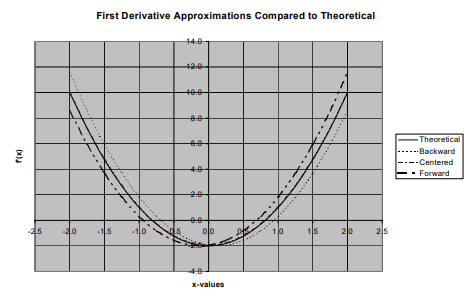
\includegraphics[width=0.8\linewidth]{fig_4_2}
		\label{fig:fig_4_2}
	\end{figure}
\bigbreak
\hspace{-1cm}
\begin{tabular}{rrrrrrrrrr}
\multicolumn{1}{l}{$\underline{\mathbf{x}}$} & $\underline{\mathbf{f}(\mathbf{x})}$ & $\underline{\mathbf{f}(\mathbf{x}-\mathbf{1})}$ & $\underline{\mathbf{f}(\mathbf{x}+\mathbf{1})}$ & $\underline{\mathbf{f}(\mathbf{x}-\mathbf{2})}$ & $\underline{\mathbf{f}(\mathbf{x}+\mathbf{2})}$ & $\underline{\mathbf{f}^{\prime\prime}(\mathbf{x}) \textbf {-Theory }}$ & $\underline{\mathbf{f}^{\prime\prime}(\mathbf{x}) \textbf {-Back }}$ & $\underline{\mathbf{f}^{\prime\prime}(\mathbf{x})-\mathbf{C e n t}}$ & $\underline{\mathbf{{f}^{\prime\prime}(}\mathbf{{x})} \textbf {-Forw }}$ \\\\
$-2.000$ & $0.000$ & $-2.891$ & $2.141$ & $3.625$ & $3.625$ & $ -12.000$ & $150.500$ & $-12.000$ & $-10.500$\\
$-1.750$ & $2.141$ & $0.000$ & $3.625$ & $-2.891$ & $4.547$ & $-10.500$ & $-12.000$ & $-10.500$ & $-9.000$\\
$-1.500$ & $3.625$ & $2.141$ & $4.547$ & $0.000$ & $5.000$ & $-9.000$ & $-10.500$ & $-9.000$ & $-7.500$ \\
$-1.250$ & $4.547$ & $3.625$ & $5.000$ & $2.141$ & $5.078$ & $-7.500$ & $-9.000$ & $-7.500$ & $-6.000$ \\
$-1.000$ & $5.000$ & $4.547$ & $5.078$ & $3.625$ & $4.875$ & $-6.000$ & $-7.500$ & $-6.000$ & $-4.500$\\
$-0.750$ & $5.078$ & $5.000$ & $4.875$ & $4.547$ & $4.484$ & $-4.500$ & $-6.000$ & $-4.500$ & $-3.000$\\
$-0.500$ & $4.875$ & $5.078$ & $4.484$ & $5.000$ & $4.000$ & $-3.000$ & $-4.500$ & $-3.000$ & $-1.500$\\
$-0.250$ & $4.484$ & $4.875$ & $4.000$ & $5.078$ & $3.516$ & $-1.500$ & $-3.000$ & $-1.500$ & $0.000$\\
$0.000$ & $4.000$ & $4.484$ & $3.516$ & $4.875$ & $3.125$ & $0.000$ & $-1.500$ & $0.000$ & $1.500$\\
$0.250$ & $3.516$ & $4.000$ & $3.125$ & $4.484$ & $2.922$ & $1.500$ & $0.000$ & $1.500$ & $3.000$\\
$0.500$ & $3.125$ & $3.516$ & $2.922$ & $4.000$ & $3.000$ & $3.000$ & $1.500$ & $3.000$ & $4.500$\\\\
$0.750$ & $2.922$ & $3.125$ & $3.000$ & $3.516$ & $3.453$ & $4.500$ & $3.000$ & $4.500$ & $6.000$\\
$1.000$ & $3.000$ & $2.922$ & $3.453$ & $3.125$ & $4.375$ & $6.000$ & $4.500$ & $6.000$ & $7.500$\\
$1.250$ & $3.453$ & $3.000$ & $4.375$ & $2.922$ & $5.859$ & $7.500$ & $6.000$ & $7.500$ & $9.000$\\
$1.500$ & $4.375$ & $3.453$ & $5.859$ & $3.000$ & $8.000$ & $9.000$ & $7.500$ & $9.000$ & $10.500$\\
$1.750$ & $5.859$ & $4.375$ & $8.000$ & $3.453$ & $10.891$ & $10.500$ & $9.000$ & $10.500$ & $12.000$\\
$2.000$ & $8.000$ & $5.859$ & $10.891$ & $4.375$ & $14.625$ & $12.000$ & $10.500$ & $12.000$ & $13.500$\\
\end{tabular}
\bigbreak
\begin{figure}[H]\quad\quad\quad\quad\quad\quad\quad\quad\quad
		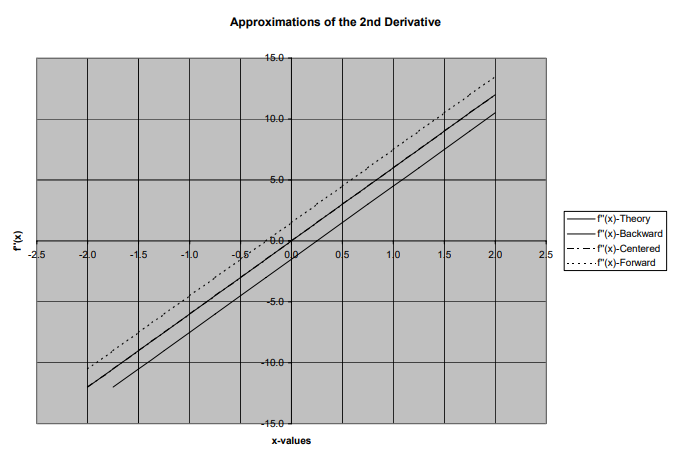
\includegraphics[width=0.75\linewidth]{fig_4_3}
		\label{fig:fig_4_3}
	\end{figure}
\bigbreak


\section{}
\begin{lstlisting}[numbers=none]
function eps = macheps
% determines the machine epsilon
e = 1;
while e+1>1
  e = e/2;
end
eps = 2*e;

>> macheps

ans =
 2.2204e-016
 
>> eps

ans =
 2.2204e-016
\end{lstlisting}

\end{enumerate}
\end{document}

